\documentclass[handout,nooutcomes]{ximera}
\usepackage{booktabs}
%% handout
%% space
%% newpage
%% numbers
%% nooutcomes

\renewcommand{\outcome}[1]{\marginpar{\null\vspace{2ex}\scriptsize\framebox{\parbox{0.75in}{\begin{raggedright}P\arabic{problem} Outcome: #1\end{raggedright}}}}}

\renewenvironment{freeResponse}{
\ifhandout\setbox0\vbox\bgroup\else
\begin{trivlist}\item[\hskip \labelsep\bfseries Solution:\hspace{2ex}]
\fi}
{\ifhandout\egroup\else
\end{trivlist}
\fi}

\newcommand{\RR}{\mathbb R}
\renewcommand{\d}{\,d}
\newcommand{\dd}[2][]{\frac{d #1}{d #2}}
\renewcommand{\l}{\ell}
\newcommand{\ddx}{\frac{d}{dx}}
\everymath{\displaystyle}
\newcommand{\dfn}{\textbf}
\newcommand{\eval}[1]{\bigg[ #1 \bigg]}


\title{Breakout Session 7: Introduction to derivatives}  

\begin{document}
\begin{abstract}
  \textbf{A look back:} In the previous (January 28, 2016) Breakout Session you practiced how to interpret and apply the definition of continuity, the intermediate value theorem, and how to determine intervals of continuity.

  \textbf{Overview:} In today's (February 2, 2016) Breakout Session you will resume the study of rates of change and the relationship between rates of change and graphs of famous functions.

  \textbf{A look ahead:} In the next (February 4, 2016) Breakout Session you will start to understand the connection between the graph of a derivative and its corresponding (famous) function and discuss the three ways a function is \emph{not} differentiable at a point.
\end{abstract}
\maketitle

\section{Learning Outcomes}
\label{section:learning-outcomes}
The following outcomes are \emph{not an exhaustive} list of the skills you will need to develop and integrate for demonstration on quizzes and exams.
This list is meant to be a starting point for conversation (with your Lecturer, Breakout Session Instructor, and fellow learners) for organizing your knowledge and monitoring the development of your skills.
\begin{itemize}
  \item
    Use limits to find the slope of the tangent line at a point.

  \item
    Write the equation of the tangent line.
    
  \item
    Find the derivative function using the limit definition.

  \item
    Understand the difference between average and instantaneous velocity.

  \item
    Understand secant and tangent lines.

  \item
    Understand the definition of the derivative at a point. 

  \item 
    Understand the derivative as a function. 
\end{itemize}

\newpage
\begin{problem}
  \label{problem:vertical-tangent-line}
  Define the function $f$ by $f(x) = x^{1/3}$ and consider the graph of this function:
  \begin{image}
    \includegraphics[scale = 0.5]{Images/"Graph for warmup".png}
  \end{image}

  Which of the following two statements are true:
  \begin{itemize}
    \item[(a)]
      The graph of $f$ has a tangent line at $x = 0$.
    \item[(b)]
      The derivative $f'(0)$ is defined.
  \end{itemize}
\end{problem}

\begin{problem}
  \label{problem:two-different-characterizations}
    Recall the following two graphs from:
  \[
    \begin{array}{lr}
      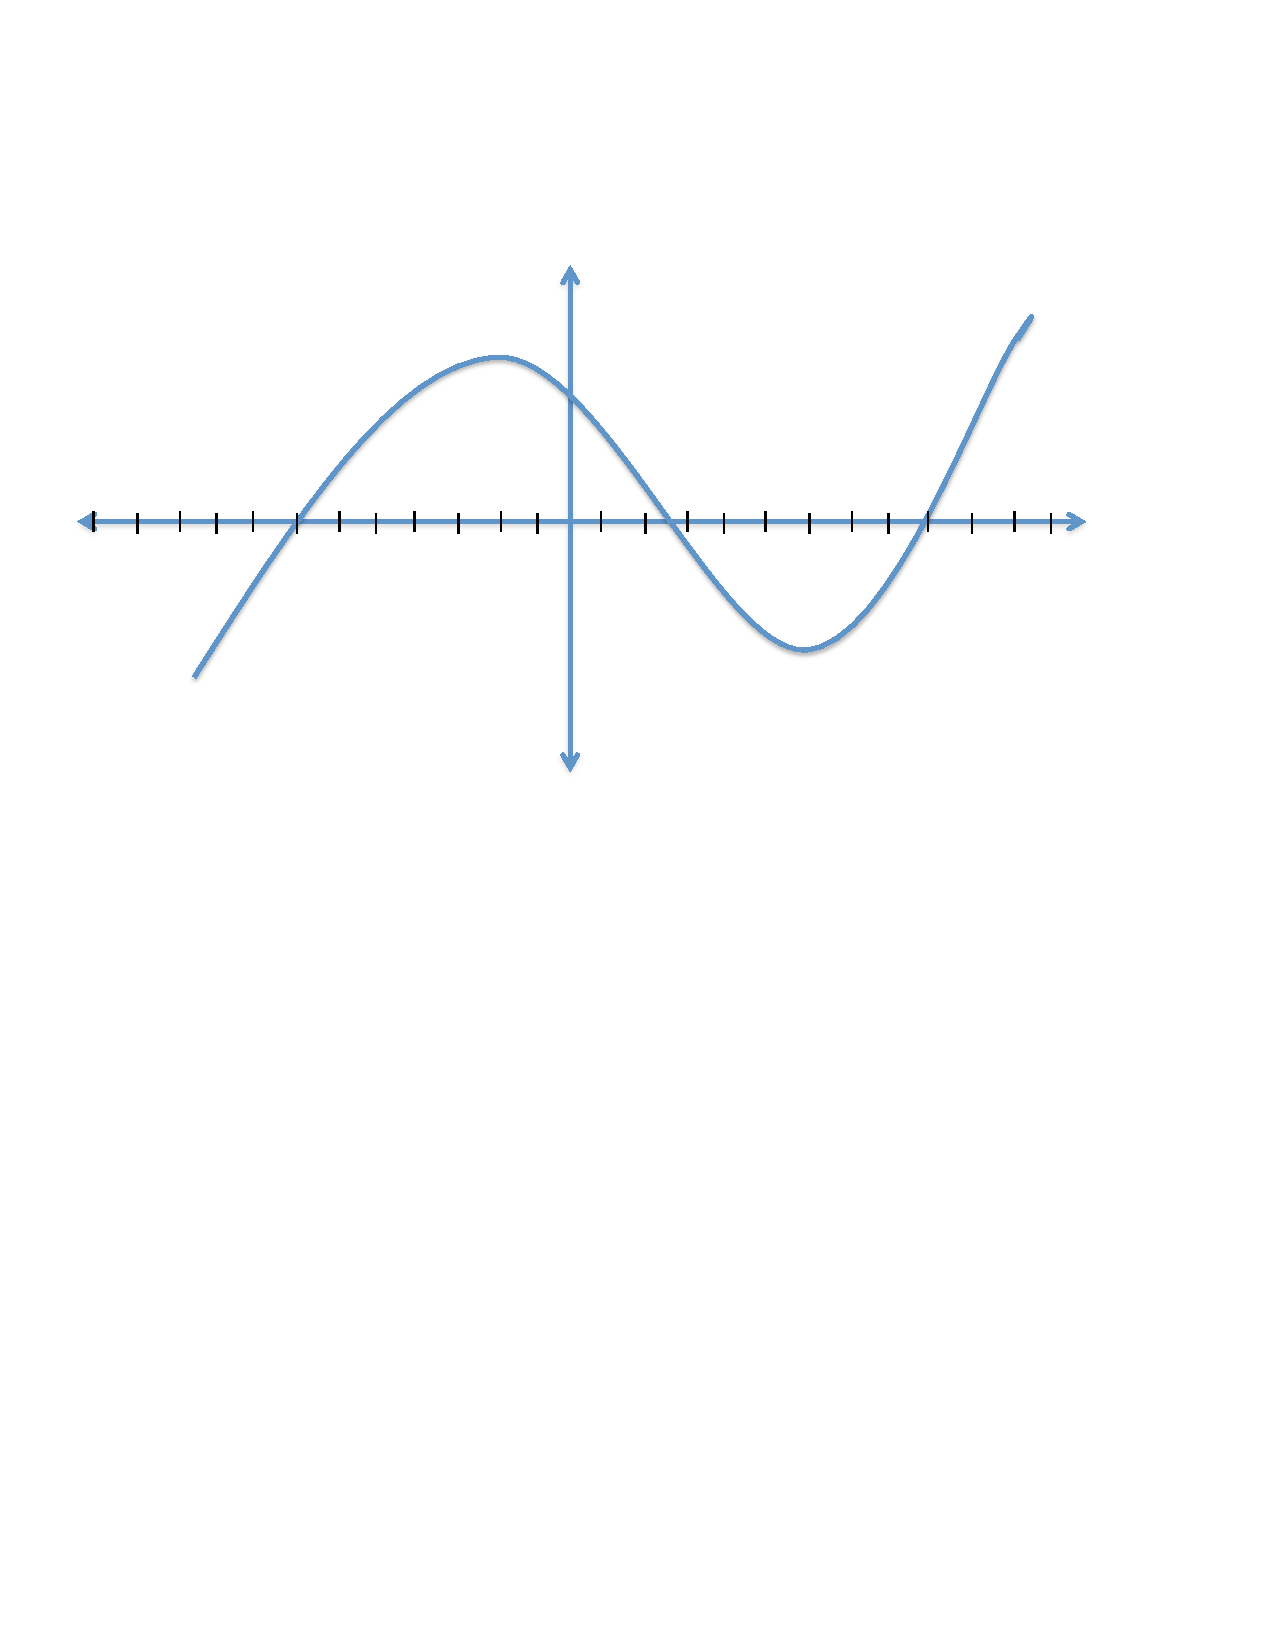
\includegraphics[trim= 150 350 250 180]{Images/Figure2.pdf} &		   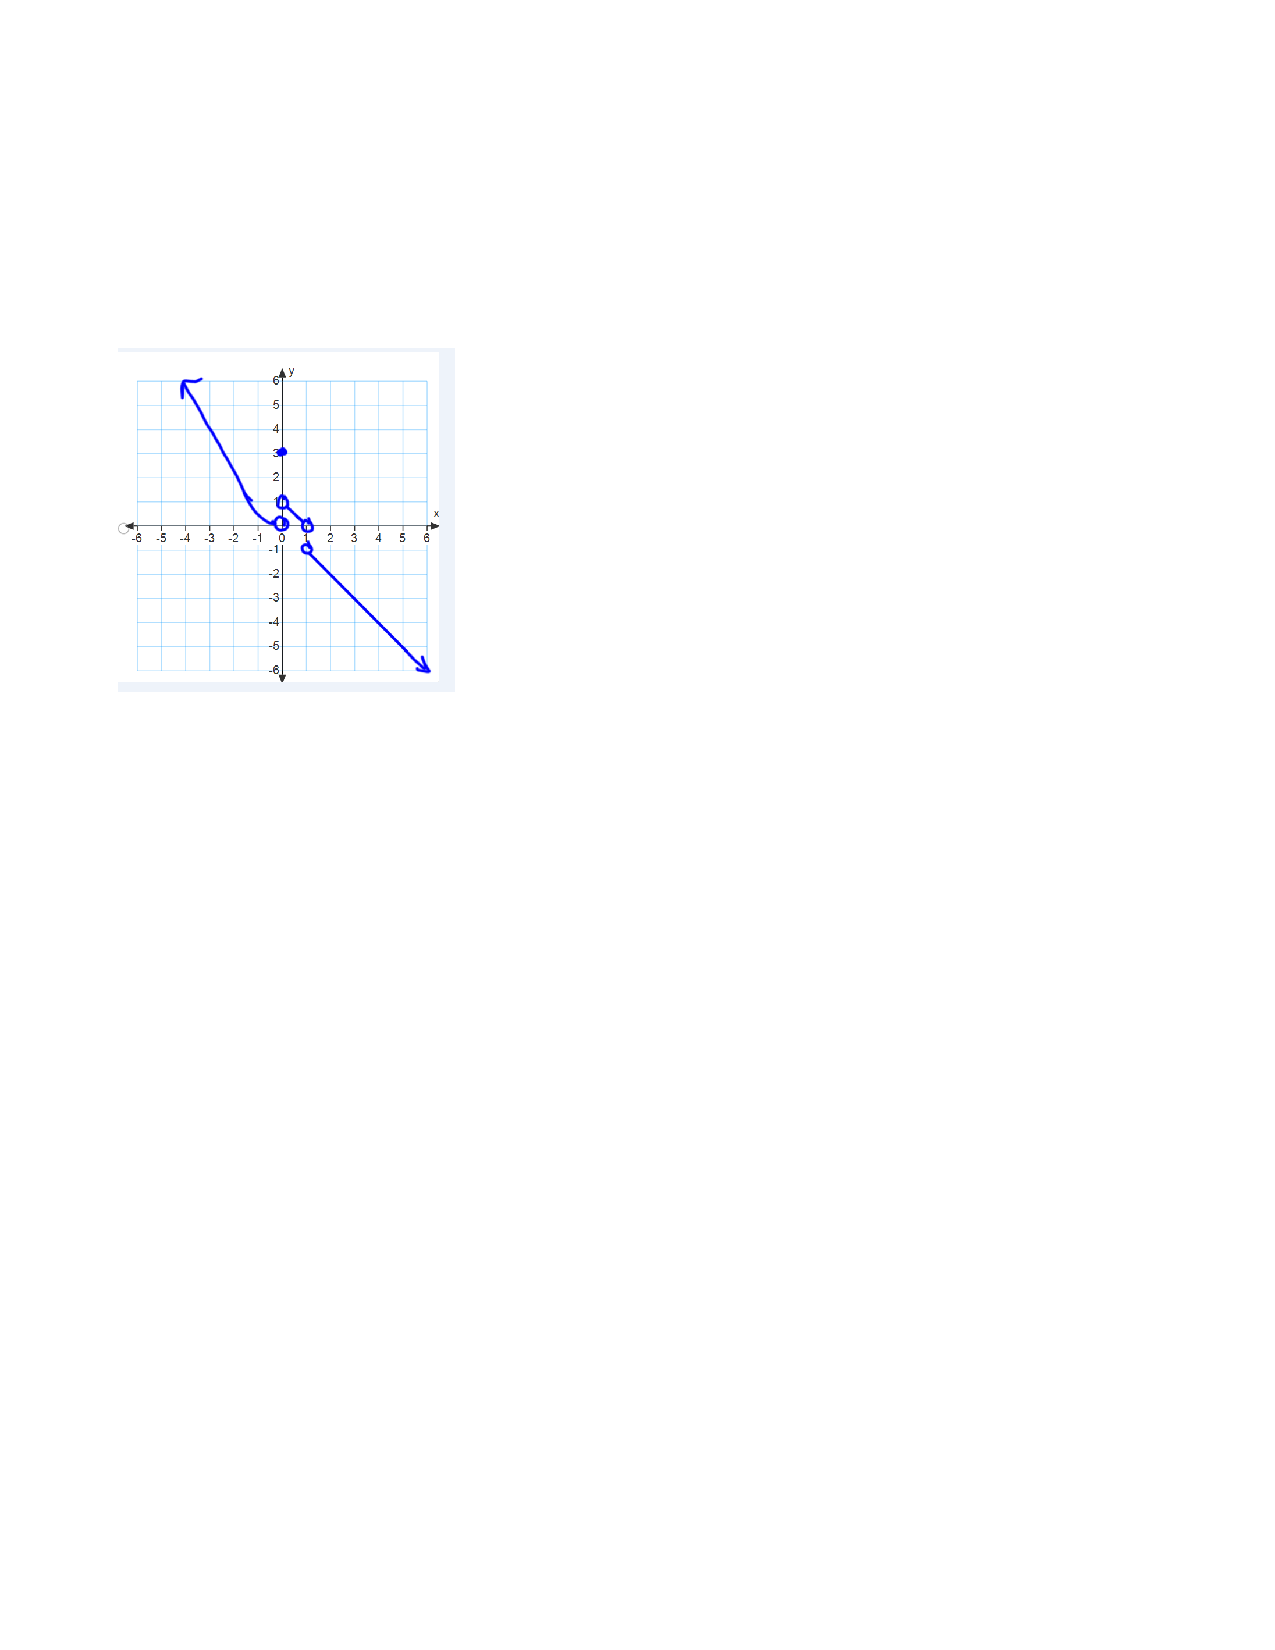
\includegraphics[trim= 140 350 250 180]{Images/Figure3.pdf}
    \end{array}
  \]
  \begin{itemize}
    \item
      What are the similarities between the two graphs?
    \item 
      What are the differences?
    \item 
      Why is one notation different from the other notation in the graphs?
    \item 
      For each of the two graphs, which lines are the secant lines?
    \item 
      For each of the two graphs, which lines are the tangent lines?
    \item 
      What is the main concept these graphs are trying to communicate?
  \end{itemize}
\end{problem}

\begin{problem}
  \label{problem:find-equation-of-tangent-line}
    For each of the following functions find the equation of the tangent line at the given point.
  \begin{itemize}
    \item[(a)]
      $h(x) = -5x^2 + 7x - 9$ at $x = 3$.

    \item[(b)]
      $g(u) = \sqrt{5u-4}$ at $u = 3$.

    \item[(c)]
      $\displaystyle s(z) = \frac{z}{z-5}$ at $z = 3$.
  \end{itemize}
\end{problem}

\begin{problem}
  \label{problem:nondifferentiable-at-point}
   Define the function $f$ by $f(x) = |5-x|$.
  \begin{itemize}
    \item[(a)]
      Find $f'(5)$.

    \item[(b)]
      For $a < 5$, find $f'(a)$.

    \item[(c)]
      For $a > 5$, find $f'(a)$.
  \end{itemize}

\end{problem}
\end{document} 
